\subsection{Analysis and restarting with haMSMs: NTL9 Protein Folding}

\subsubsection{Introduction}
Although the WE strategy provides an efficient framework for unbiased rare-event sampling, slow relaxation to steady state and impractically large variance in rate constant estimates may still be limiting factors for complex systems.
History-augmented Markov state models (haMSMs) have been demonstrated to provide estimates of steady state from transient, relaxation-phase WE data, which can be used to start new WE simulations \citep{copperman_accelerated_2020}. 
As shown in \textbf{Figure 6}, the haMSM plugin for the WESTPA 2.0 software package automatically constructs an haMSM from one or more independent WE simulations to estimate steady-state observables and then can automatically initiate new simulations from those estimates and iteratively repeat this procedure when those simulations complete. 
The underlying haMSM analysis library, \verb|msm_we|, can also be used to perform stand-alone haMSM analysis of existing WESTPA data.

\textbf{Learning Objectives.}  This tutorial demonstrates the use of an haMSM restarting workflow in WE simulations of the ms-timescale folding process of the NTL9 protein. 
Specific objectives are:
\begin{enumerate}
    \item How to apply the haMSM plugin for periodic restarting of simulations;
    \item How to use the \verb|msm_we| package to build an haMSM from WE data;
    \item How to estimate the distribution of first passage times from the haMSM, using \verb|msm_we|.
\end{enumerate}

\subsubsection{Prerequisites} The Basic and Intermediate WESTPA Tutorials \citep{bogetti_suite_2019} should be completed before running this tutorial.

\textbf{Computational Requirements.} This tutorial can be completed on a computer with a single GTX1080 GPU and a 2.4GHz Xeon E5-2620 in 90 min. 
The WE simulation will generate \textasciitilde5 GB of data, though on a typical cluster filesystem, overhead associated with data redundancy may increase this to \textasciitilde15 GB. 
A version of the Amber software package compatible with Amber 16 restart and topology files must be installed to propagate the dynamics and calculate the WE progress coordinate. 

The \verb|msm_we| Python package must also be installed, which can be done by first cloning the repository and then installing it into your existing conda environment (with WESTPA already installed) by running:
\begin{verbatim}
  $ git clone https://github.com/westpa/msm_we
  $ cd msm_we 
  $ conda env update --name <your WESTPA conda env> 
          --file environment.yml
\end{verbatim}

\begin{figure}[t]
\centering
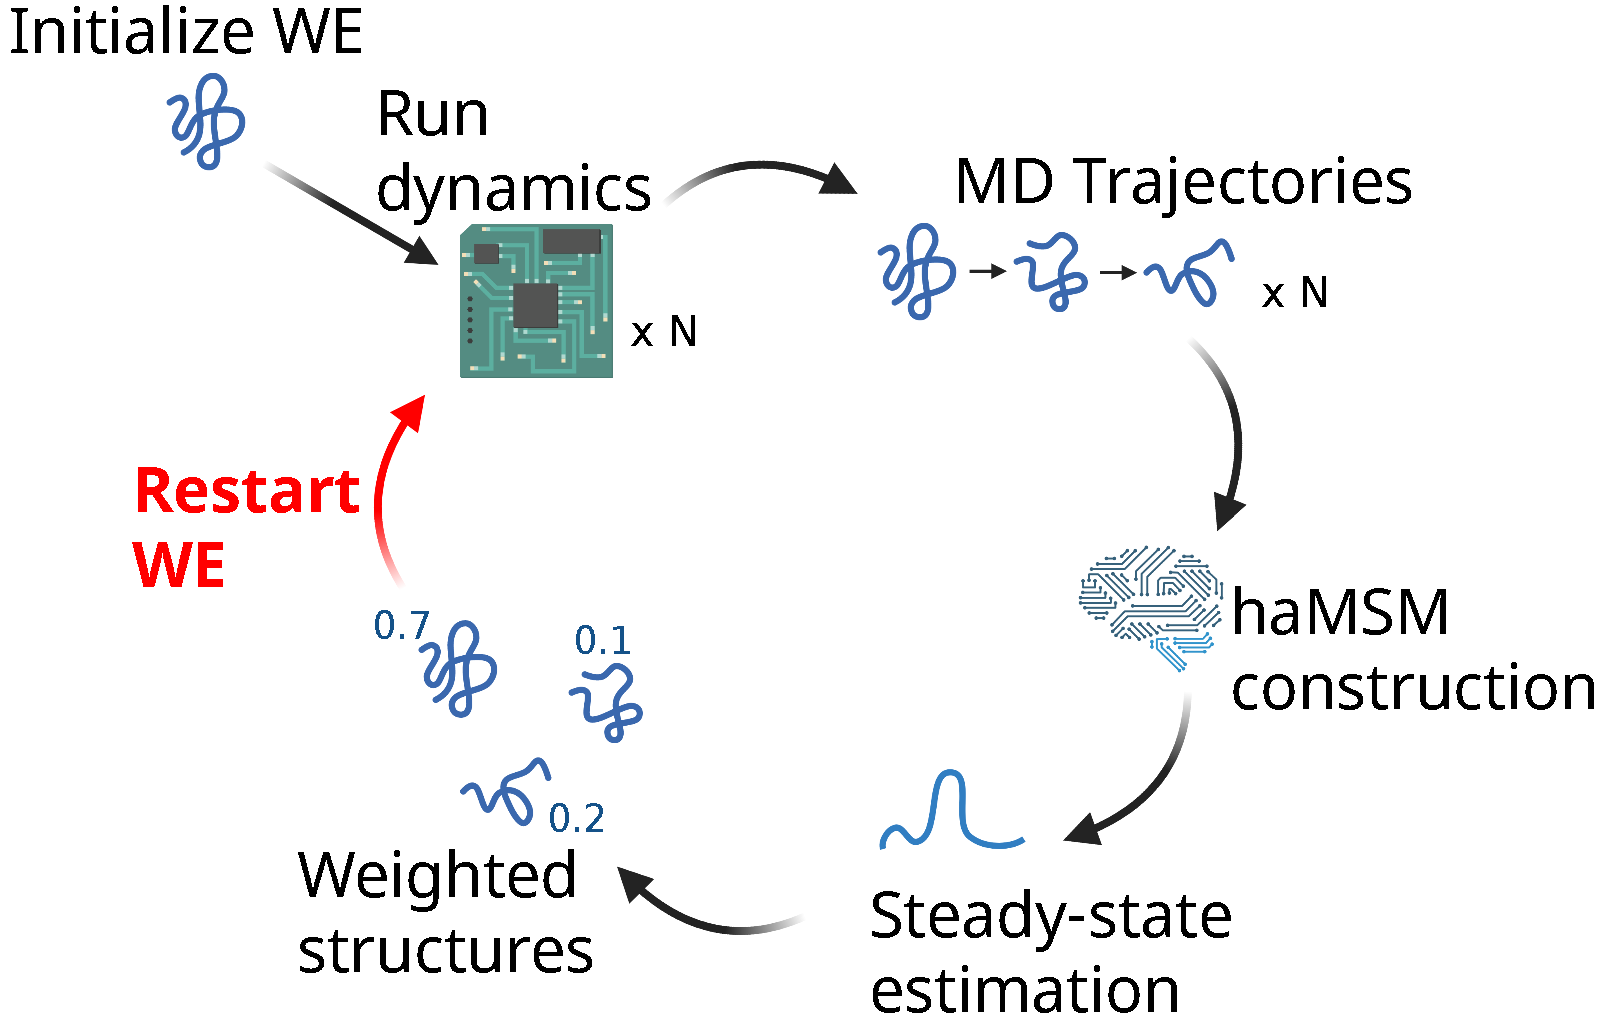
\includegraphics[width=\columnwidth]{figures/Figure6_haMSM.pdf}
\caption{Schematic of haMSM restarting procedure. 
Trajectories from one or more WE runs are used together to build an haMSM. 
An estimate of steady-state is obtained from the haMSM, and is used to assign weights to all sampled structures. 
New WE runs are initiated from these steady-state weighted structures, and the procedure repeats. 
Figure reprinted with permission from \citep{russo_westpa_2022}. 
Further permission related to the source material should be requested from ACS.}
\end{figure}

\subsubsection{Plugin functionality}
Once we initiate a WESTPA run with the haMSM plugin enabled, the plugin will execute a series of independent WE simulations (runs) from the same starting configuration for the number of WE iterations specified in \verb|west.cfg|. 
For this tutorial, the runs will not use the HDF5 trajectory-saving framework.

If none of the WE runs have reached the target state, the haMSM plugin will sequentially extend each run for a number of iterations specified in \verb|west.cfg|. 
This extension procedure will be repeated until at least one run has reached the target state. 
For consistency, all of the other runs in the set will be extended to match the length of this run. 
As a result of this extension procedure, runs used for the first restart may be longer than runs in subsequent restarts.

After completing the extension procedure, the plugin will construct an haMSM from these runs, and estimate the steady-state distribution and flux into the target state. 
All structures sampled by the set of runs are used to build this haMSM, and are then weighted according to a steady state. 
Note that this haMSM uses only the first and last frame of each WE iteration, which effectively sets the lag-time equal~ to~ the~ WE~ resampling~ time. A~ number of~ plots~ are~ automatically generated from the model. 
The flux profile, shown in \textbf{Figure 7}, provides an important metric of convergence, and should be examined carefully. 
A flatter flux profile indicates more converged weighted ensemble.

\begin{figure}[ht]
    \centering
    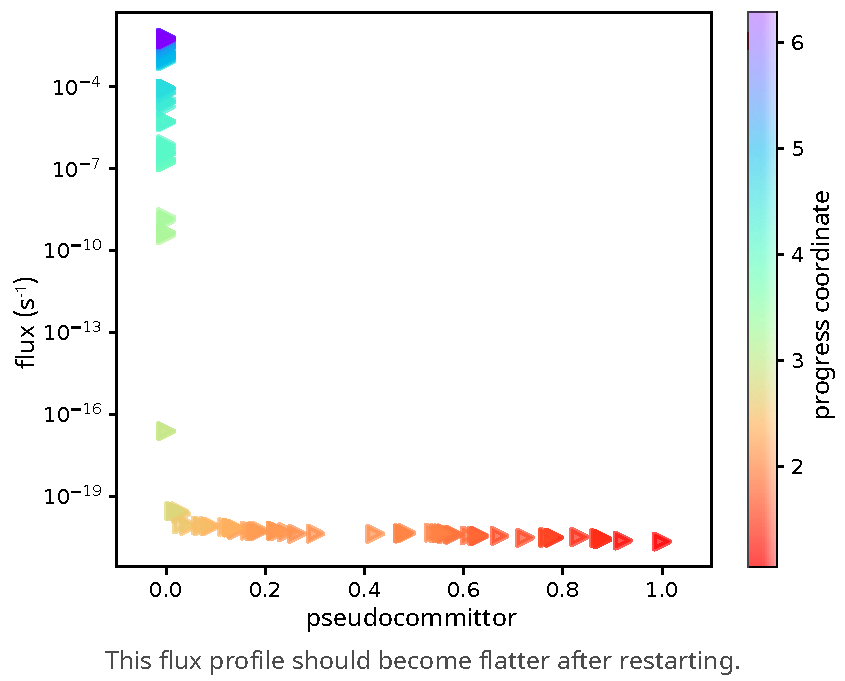
\includegraphics[width=\columnwidth]{figures/Figure7_committor.pdf}
    \caption{Sample flux profile generated by haMSM restarting plugin after a restart. 
    The x-axis is labeled "pseudocommittor", since these are committor values generated from a unidirectional path ensemble. 
    This plot should flatten in successive restarts until steady state is reached.
    The color scale indicates the progress coordinate associated with each pseudocommittor---notably, most of the dynamic range in committor-space is restricted to a small range of progress coordinate values. 
    This image can be found in restart0/plots/psuedocomm-flux\_plot\_pcoordcolor.pdf after restart is performed.}
\end{figure}

A new set of (correlated, but independent from this point onward) runs is initialized from those weighted structures. 
As a technical note, when initializing the new WE simulations, these structures are used as "start states". 
Within the WESTPA 2.0 framework, start states are a third category of state, in addition to basis states and target states. 
Like basis states, start states are used for seeding trajectory walkers when initializing a simulation with \verb|w_init|; however, \textit{unlike} basis states, they are not used after this point and walkers reaching the target state will \textbf{not} be recycled into start states but rather only to the basis states. 
The new WE runs are executed for the number of WE iterations specified in \verb|west.cfg|, in series. 
At this point, the model is saved, a new restart is prepared, and the process repeats from that point onward.

Please see \citep{russo_westpa_2022, copperman_accelerated_2020} for more theoretical background on the models used by this plugin.

\subsubsection{Preparing the system}

\noindent\textbf{The system.} For our simulation of the NTL9 protein folding process, we use a stochastic Langevin thermostat with low-friction (collision frequency $\gamma$ = 5 ps\textsuperscript{-1}) and a generalized Born implicit solvent model. 
The system consists of \textasciitilde600 atoms. 
We will use the haMSM restart plugin to automatically perform three independent WESTPA runs serially before constructing an haMSM. 
A single restart will be performed from the haMSM steady state estimate, and then WE simulation will be continued for another 106 WE iterations for each of the three runs.

To reduce runtime for this tutorial, we provide a partially completed set of three independent WE simulations. 
In this set of simulations, the first two runs have completed, and the third is nearing completion. 
None of these simulations have yet reached the target state. 

After continuing this set of WE simulations, the third simulation will finish and reach its maximum number of WE iterations. 
With very high probability, none will have reached the target folded state, and pre-restart extensions will be triggered. 
The initialized runs were chosen such that it is unlikely that the third run will reach the target state before the next restart. 
However, it is possible that in the remaining few WE iterations of the third simulation, this simulation will reach the target state, in which case we will skip the extension procedure.

After a single round of extensions, the target state should be reached in run 2, though not necessarily runs 1 or 3. 
We will construct the haMSM from the three extended runs, and restart a new set of three runs from the steady-state estimates.

\textbf{Structure of Plugin-Specific Files.} The following is a list of some important files used and generated in \verb|$WEST_SIM_ROOT/| by the haMSM plugin.


\begin{verbatim}
./restart.dat            [Tracks current restart/run]
./restart_initialization.json [User provided on 
                start, modified by plugin during run]
./west.h5  [Generated by WESTPA for the currently 
                                          active run]
./restart0/ [Stores data from the first restart. 
                                          0-indexed.]
  ./JtargetSS.txt [haMSM target steady-state 
                                       flux estimate]
  ./pSS.txt [haMSM steady-state 
                               distribution estimate]
  ./hamsm.obj         [Pickled msm_we.ModelWE object]
  ./startstates.txt  [Used for next 
              restart, holds all weighted structures]
  ./basisstates.txt  [The initial set of 
                     basis states supplied to w_init]
  ./targetstates.txt  [The initial set of 
                    target states supplied to w_init]
  ./structs/  [Complete set of structure 
             files for all structures in startstates]
  ./run*/  [Backed up traj_segs, seg_logs, and 
              west.h5 from each run in this marathon.
                                          1-indexed.]
  ./plots/[*].pdf      [Various auto-generated plots]
./restart*/                          [Other restarts]


\end{verbatim}

The following files containg more adjustable parameters or are more tightly integrated in the workflow and therefore warrant a more in-depth explanation.

\verb|west.cfg|: The haMSM restarting plugin requires a number of parameters to be set in the appropriate section of \verb|west.cfg|. 
Details regarding these parameters are listed at {\url{https://westpa.readthedocs.io/en/latest/documentation/ext/westpa.westext.hamsm_restarting.html#west-cfg}}.

\verb|restart_initialization.json|: When initializing each run, the plugin needs to know what configuration it should be launched with. 
After the first restart, this is automatically generated. 
However, \textit{before} the first restart (i.e. in producing the initial set of runs in Workflow Step 1), there is no way for the plugin to determine how the first run was initialized. 
So, the parameters initially passed to \verb|w_init| must be manually entered into \verb|restart_initialization.json|.

\verb|westpa_scripts/restart_overrides.py|: When building the haMSM, some dimensionality reduction is typically necessary as it's generally neither practical nor useful to analyze the model on the full set of coordinates. 
This dimensionality reduction is highly system-specific, so no general procedure is distributed with the plugin. 
Instead, the user is required to define a function which takes in an array of full-atomic coordinates of shape \verb|(n_segments, n_atoms, 3)|, perform the desired dimensionality reduction, and then return the reduced coordinates in an array of shape \verb|(n_segments, n_features)|. 
This functions are then loaded by the haMSM analysis code at run-time, and used throughout. 
More details are available at {\url{https://westpa.readthedocs.io/en/latest/documentation/ext/westpa.westext.hamsm_restarting.html#featurization-overrides}}.

\textbf{Preparing the WE Simulation Environment.} To prepare the system for using the haMSM restarting plugin, first clone the tutorial repository. 
In \verb|env.sh|, change \verb|TEMPDIR_ROOT| to point to a directory on your filesystem where temporary files will be created (on a cluster, this should ideally be some node-local scratch/temp space that supports I/O, but on a local workstation can be a new folder such as \verb|$WEST_SIM_ROOT/temp|). 
This temp space will be used for temporary files created during progress coordinate calculation. 
In the same file, change \verb|AMBER_EXEC| and \verb|CPPTRAJ| to point to your AMBER and CPPTRAJ executables. 
In \verb|west.cfg|, change \verb|ray_tempdir| to point to the same directory as \verb|TEMPDIR_ROOT|. 
Then examine haMSM plugin-specific configuration files above to familiarize yourself with them, though for this tutorial, no further changes are required. 
To download and extract the prepared files for the in-progress simulation this tutorial uses, run the following command from within the main simulation directory.

\begin{verbatim}
  $ bash pull_sample_data.sh
\end{verbatim}

\subsubsection{Running the WE simulation}
Now, we are ready to (re)start the WE simulation. 
The haMSM plugin will automatically perform the restarting and analysis. Typically, we would initialize the system using \verb|w_init| as we do for all WE simulations using the WESTPA 2.0 software package. 
However, to reduce the runtime for this tutorial, we have provided a pre-prepared system, and running \verb|w_init| is not required. 
Once we have configured the haMSM plugin through \verb|west.cfg|, we can restart the WE simulation and run the simulation for a few iterations, by simply executing the following command.

\begin{verbatim}
  $ ./run.sh
\end{verbatim}

If the target state has not been reached after running for the specified number of iterations, additional rounds of restarting/extending the WE simulation will automatically be launched. 
Once the target state has been reached, the plugin will build an haMSM, update statistical weights for each sampled structure, and restart a new set of WE trajectories initialized from those structures with updated weights. 
This will all be done automatically.

\textbf{Start States.} After performing a restart, we will find under the \verb|restart0/| directory a \verb|startstates.txt| reference file that lists all the structures used for the restart (start states) and their associated weights for initializing new WE simulations from the first round of restarting. 
As noted, these are distinct from the basis states. 
The \verb|startstates.txt| text file is formatted with three columns, which define the names (e.g., “b21s0”), associated probabilities, and name of the directory containing the structure files of the start states (relative to the path defined under \verb|west.data_refs.basis_states| in \verb|west.cfg|). 
Structure files corresponding to these start states are in \verb|restart0/structs/| and are named according to the structure’s haMSM bin and the structure’s index within that bin. 
Start states can be added to the pool of potential structures for WE initialization by adding the \verb|--sstates-from| or \verb|--sstates| option to the \verb|w_init| command. 
Similar to the \verb|--bstates| options for basis states in the above \textbf{Advanced Tutorial 3.1}, the \verb|--sstates-from| option is used to indicate a text file with a list of start states and the \verb|--sstates| option is used to append additional start states through the command line.

\subsubsection{Analyzing the WE simulation}
After the plugin finishes running, you will find the associated \verb|west.h5| for each run and the associated haMSM pickled \verb|hamsm.obj| objects for each marathon in the \verb|restart*/| directories. 
Although the plugin will automatically build the haMSMs and perform some of the analysis based on the configuration files, haMSM analysis can also be manually performed post-simulation on WESTPA data with the \verb|msm_we| library (as used internally by the plugin).

For this tutorial, you can use either the data generated by the steps above, or the pre-prepared \verb|west.h5| files containing data generated from a similar simulation configuration. 
This analysis largely follows the \verb|msm_we| usage instructions provided in the \verb|msm_we| documentation ({\url{https://jdrusso.github.io/msm_we/usage.html}}).

For detailed instructions on how to analyze your simulation results, please refer to the Jupyter notebook distributed along with this tutorial.

\subsubsection{Conclusion}
Complex systems may exhibit relaxation slow enough to prevent direct measurement of rate constants using probability flux in WE. 
This tutorial therefore presents the haMSM plugin for leveraging relaxation-phase WE simulations by automatically (i) building a haMSM; (ii) generating an estimate of the steady-state probability distribution and the corresponding steady flux; and (iii) if desired, restarting a new WE simulation or set of simulations from the estimated steady state. 
Each haMSM yields an estimate for the MFPT and FPT distribution using \verb|msm_we|.